\section{Experiment}
\subsection{Implementation Details}
We use pretrained Wan2.2-5B~\cite{wan2025} as the backbone, including its video DiT, text encoder, and video VAE. The action expert shares the same architecture as the video branch but uses a reduced hidden dimension of $d_a=1024$, resulting in a 1B action expert and a total model size of 6B parameters. We set the action horizon to $h=32$. Video frames are temporally downsampled by $4\times$, resulting in 9 video frames per chunk. Images from multiple cameras are concatenated into a single image before being fed into the VAE.

We use the same flow-matching formulation for both the video and action branches. Following~\cite{wan2025}, we adopt a logit-normal distribution over $t$ as the noise schedule during both training and inference. During inference, we use 10 denoising steps with classifier-free guidance (CFG) scale set to 1.0. We use AdamW with a learning rate of $1\times10^{-4}$, weight decay of 0.01, and a cosine annealing schedule for all training settings. Training is conducted in mixed precision with gradient clipping at 1.0. All latency numbers are measured on a single NVIDIA RTX 5090D V2 32GB GPU.

We build Fast-WAM-Joint by allowing attention between video and action tokens. For Fast-WAM-IDM, we follow~\cite{lingbot-va2026} and apply noise augmentation to the ground-truth video tokens with probability $p=0.5$.



\subsection{Experiment Setup}
We evaluate Fast-WAM and its variants on both simulation benchmarks, namely LIBERO~\cite{liu2023libero} and RoboTwin 2.0~\cite{chen2025robotwin}, as well as on a real-world manipulation task.

\paragraph{LIBERO.}
We follow the standard benchmarking protocol and train our models on the four LIBERO suites: LIBERO-Spatial, LIBERO-Object, LIBERO-Goal, and LIBERO-Long. Each suite contains 500 demonstrations spanning 10 tasks. All models are trained for 20k steps. We report success rates for each suite, evaluated over a total of 2000 trials across 40 tasks with different random seeds.

\paragraph{RoboTwin 2.0.}
RoboTwin 2.0 is a challenging bimanual manipulation benchmark featuring more than 50 tasks that require coordinated dual-arm control. We follow the multi-task training setup of~\cite{bi2025motusunifiedlatentaction, lingbot-va2026}, where models are trained on a mixture of 2,500 demonstrations collected in clean scenes and 25,000 demonstrations collected under heavy scene randomization, spanning over 50 tasks. All models are trained for 30k steps. We report average success rates over 100 trials per task under both clean and randomized settings.

\begin{figure*}[tbp]
        \centering
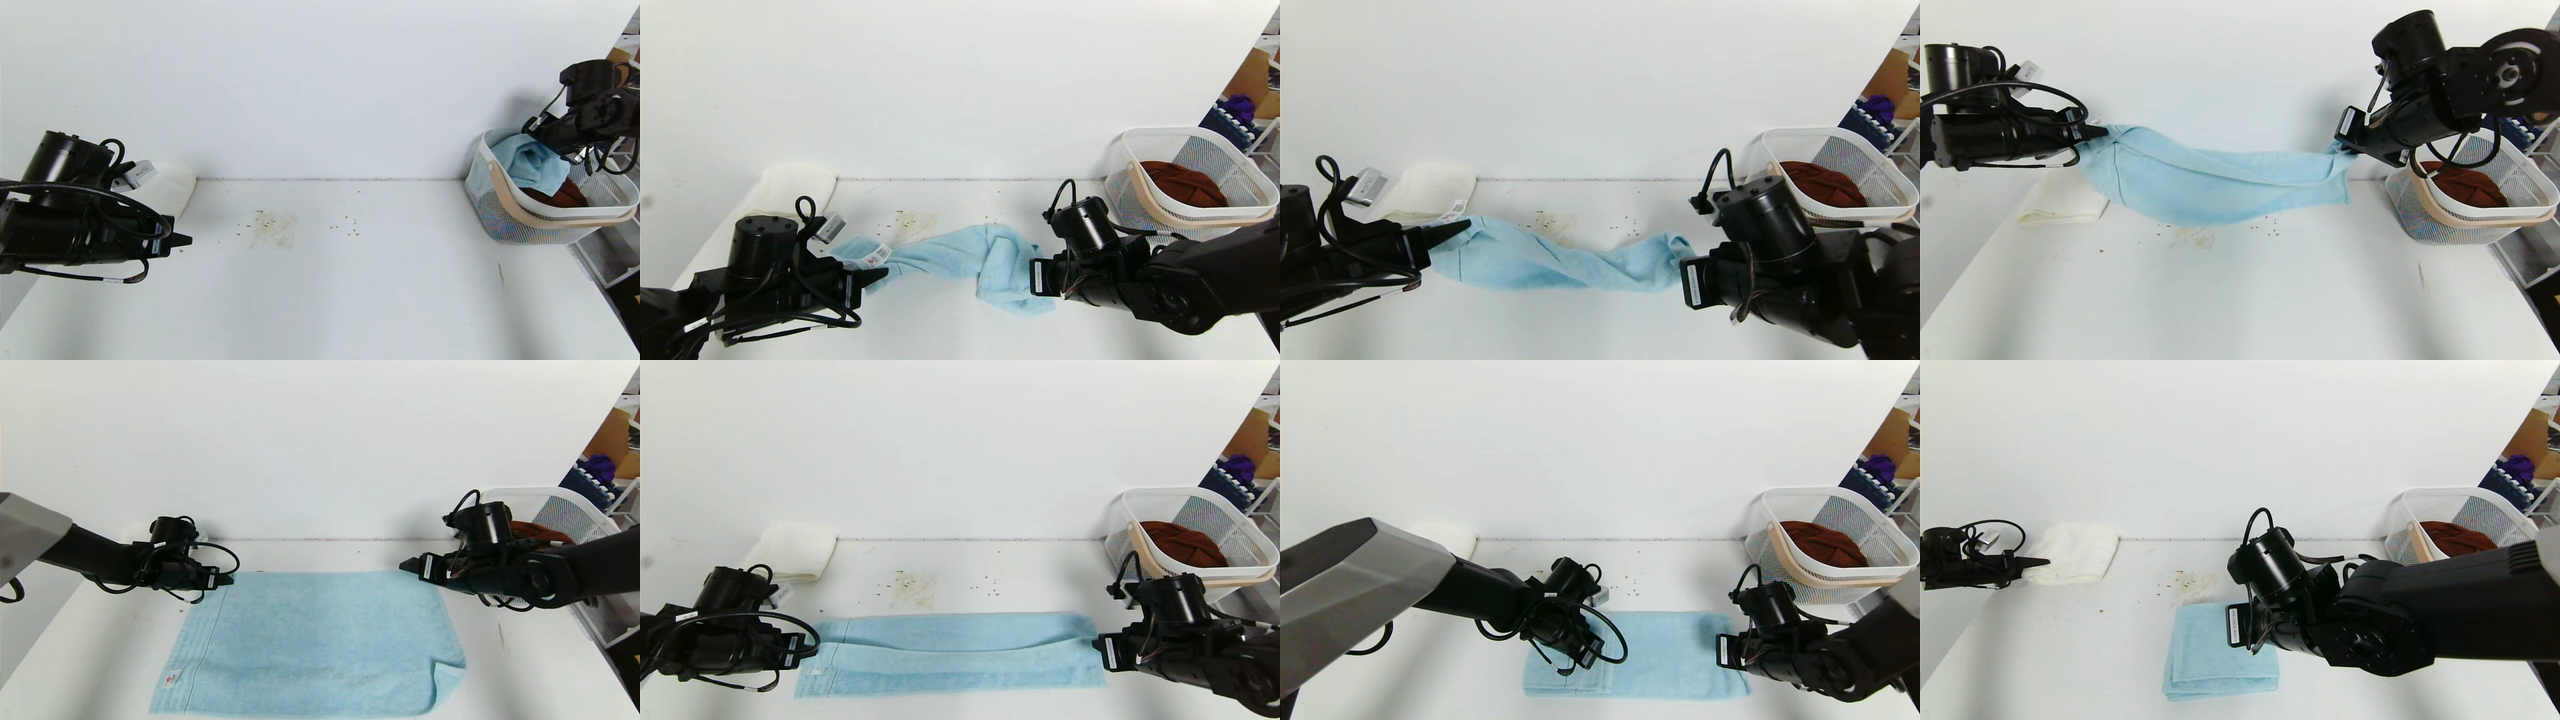
\includegraphics[width=1.0\textwidth]{figs/bench_grid_2560x720.png} 
    \caption{Real-world towel-folding task on the Galaxea R1 Lite platform. Folding a deformable object requires long-horizon planning and precise closed-loop manipulation, making it a challenging benchmark for evaluating both task success and execution efficiency.}
    \label{fig:fold_bench}
\end{figure*}

\paragraph{Real-World Evaluation.}
We conduct real-world evaluation on towel folding, a long-horizon and challenging task that requires the policy to reason about the dynamics of deformable objects, as shown in Figure~\ref{fig:fold_bench}. We collect 60 hours of teleoperated demonstrations on the Galaxea R1 Lite platform. All models are trained for 30k steps. We report both the average success rate and the average completion time. The former measures whether the policy can eventually complete the folding task given sufficient time, while the latter reflects whether the policy learns an efficient execution strategy rather than relying on repeated trial-and-error corrections. For this task, completion time is therefore as important as success rate in assessing policy quality.

\subsection{Main Results}
\subsubsection{Overall comparison on simulation benchmarks}

\begin{table}[t]
\centering
\small
\caption{Results on RoboTwin. Fast-WAM matches strong pretrained WAM baselines without using embodied pretraining, while the two imagine-then-execute variants remain highly comparable and removing video co-training causes a substantial drop.}
\label{tab:robotwin}
\resizebox{0.8\columnwidth}{!}{
\begin{tabular}{l|c|cc|c}
\toprule
Method & Embodied PT. & Clean & Rand. & \textbf{Average} \\
\midrule
% X-VLA & \cmark & 72.80 & 72.84 & 72.8 \\
$\pi_{0}$~\cite{black2024pi_0} & \cmark & 65.92 & 58.40 & 62.2 \\
$\pi_{0.5}$~\cite{intelligence2025pi_} & \cmark & 82.74 & 76.76 & 79.8 \\
Motus~\cite{bi2025motusunifiedlatentaction} & \cmark & 88.66 & 87.02 & 87.8 \\
Motus from WAN2.2 & \xmark & 77.56 & 77.00 & 77.3 \\
LingBot-VA~\cite{lingbot-va2026} & \cmark & 92.90 & 91.50  & \textbf{92.2} \\
LingBot-VA from WAN2.2 & \xmark & 80.60 & -- & 80.6 \\
\textbf{Fast-WAM (Ours)} & \xmark & 91.88 & 91.78 & \underline{91.8} \\
\midrule
\multicolumn{5}{l}{\textit{Fast-WAM Variants}} \\
\cmidrule(lr){1-5}
Fast-WAM & \xmark & 91.88 & 91.78 & \textbf{91.8} \\
Fast-WAM-Joint & \xmark & 90.84 & 90.32 & 90.6 \\
Fast-WAM-IDM & \xmark & 91.16 & 91.34 & \underline{91.3} \\
Fast-WAM w.o. video co-train & \xmark & 82.76 & 84.80 & 83.8 \\
\bottomrule
\end{tabular}
}
\end{table}

\begin{table*}[t]
\centering
\small
\caption{Results on LIBERO. Fast-WAM achieves competitive overall performance without embodied pretraining, remains close to both imagine-then-execute variants, and outperforms the no-video-co-training ablation by a clear margin.}
\label{tab:libero}
\resizebox{0.95\textwidth}{!}{
\begin{tabular}{l|c|cccc|c}
\toprule
Method & Embodied PT. & Spatial & Object & Goal & Long & \textbf{Average} \\
\midrule
OpenVLA~\cite{kim2024openvla} & \cmark & 84.7 & 88.4 & 79.2 & 53.7 & 76.5 \\
$\pi_0$~\cite{black2024pi_0} & \cmark & 96.8 & 98.8 & 95.8 & 85.2 & 94.1 \\
$\pi_{0.5}$~\cite{intelligence2025pi_} & \cmark & 98.8 & 98.2 & 98.0 & 92.4 & 96.9 \\
LingBot-VA~\cite{lingbot-va2026} & \cmark & 98.5 & 99.6 & 97.2 & 98.5 & \textbf{98.5} \\
Motus~\cite{bi2025motusunifiedlatentaction} & \cmark & 96.8 & 99.8 & 96.6 & 97.6 & \underline{97.7} \\
\textbf{Fast-WAM (Ours)} & \xmark & 98.2 & 100.0 & 97.0 & 95.2 & 97.6 \\
\midrule
\multicolumn{7}{l}{\textit{Fast-WAM Variants}} \\
\cmidrule(lr){1-7}
Fast-WAM & \xmark & 98.2 & 100.0 & 97.0 & 95.2 & 97.6 \\
Fast-WAM-Joint & \xmark & 99.6 & 99.4 & 98.2 & 96.8 & \textbf{98.5} \\
Fast-WAM-IDM & \xmark & 98.8 & 97.8 & 97.8 & 97.6 & \underline{98.0} \\
Fast-WAM w.o. video co-train & \xmark & 89.2 & 99.2 & 95.4 & 90.0 & 93.5 \\
\bottomrule
\end{tabular}
}
\end{table*}


Table~\ref{tab:robotwin} and Table~\ref{tab:libero} summarize the results on RoboTwin and LIBERO, respectively. Overall, Fast-WAM achieves performance comparable to state-of-the-art methods on both benchmarks without using embodied pretraining. Per-task results on RoboTwin are listed in Appendix Table~\ref{tab:robotwin_detail}.

On RoboTwin, Fast-WAM achieves 91.8\% success rate, exceeding all baselines without embodied pretraining and remaining highly competitive with the strongest pretrained WAMs. In particular, Fast-WAM substantially outperforms Motus~\cite{bi2025motusunifiedlatentaction} both with pretraining (87.8\%) and without pretraining (77.3\%), as well as LingBot-VA~\cite{lingbot-va2026} without pretraining (80.6\%), while remaining comparable to pretrained LingBot-VA (92.2\%). These results suggest that Fast-WAM can recover most of the benefit of prior WAM pipelines without relying on embodied pretraining.

On LIBERO, Fast-WAM also delivers strong overall performance, achieving an average success rate of 97.6\% without embodied pretraining. It outperforms the strong VLA baseline $\pi_{0.5}$ and remains competitive with pretrained WAM baselines such as LingBot-VA (98.5\%) and Motus (97.7\%). These results show that Fast-WAM is consistently effective across diverse simulation benchmarks, even without the embodied pretraining used by most prior WAM and VLA baselines.

\subsubsection{Controlled comparison with Fast-WAM variants}

We next compare Fast-WAM with the controlled variants introduced in Sec.~\ref{sec:controlled_variants} to disentangle the role of explicit future imagination at inference time from that of video co-training during training. Across both simulation benchmarks, the overall pattern is consistent: Fast-WAM remains comparable to the two imagine-then-execute variants, while removing video co-training leads to a much larger performance drop.

On RoboTwin, Fast-WAM achieves 91.8\% success rate, which is highly comparable to both Fast-WAM-Joint (90.6\%) and Fast-WAM-IDM (91.3\%). In contrast, removing video co-training reduces performance to 83.8\%, yielding a substantial gap relative to all three variants with video co-training. This result suggests that, on this benchmark, retaining the video modeling objective during training is far more important than explicitly generating future observations at test time. A similar trend holds on LIBERO. Fast-WAM reaches 97.6\% average success rate, remaining close to Fast-WAM-Joint (98.5\%) and Fast-WAM-IDM (98.0\%). By comparison, Fast-WAM without video co-training drops to 93.5\%, with especially visible degradation on the \textit{Spatial} and \textit{Long} subsets. Again, the gap caused by removing video co-training is clearly larger than the gap between Fast-WAM and the imagine-then-execute variants.

This pattern suggests that the main benefit of WAM-style training may lie less in whether, or how, future imagination is performed at test time, and more in the video prediction objective used to shape world-grounded representations during training.

\subsubsection{Real-world performance and efficiency}
\begin{figure*}[tbp]
        \centering
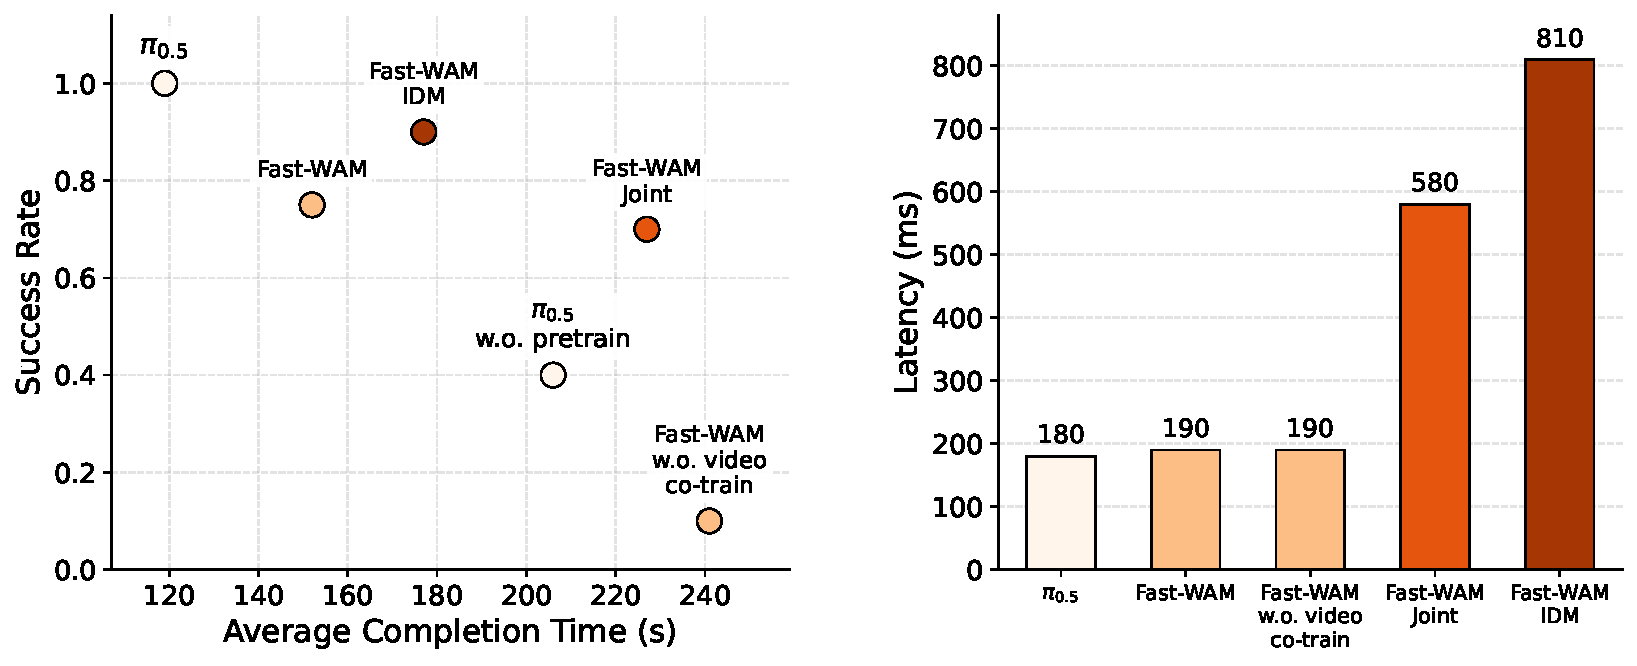
\includegraphics[width=0.95\textwidth]{figs/method_scatter_latency.pdf} 
    \caption{Real-world results on the long-horizon towel-folding task. The left panel plots success rate against average completion time, where upper-left is better. The right panel compares inference latency. Fast-WAM achieves strong real-world performance with substantially lower latency than imagine-then-execute variants, while removing video co-training degrades both success rate and completion time.}
    \label{fig:realworld_latency}
\end{figure*}
We further evaluate Fast-WAM on a long-horizon real-world towel-folding task. We report both the average success rate and the average completion time, as they capture two equally important aspects of policy quality: whether the policy can eventually complete the task, and whether it does so efficiently rather than through repeated trial-and-error corrections. Results are shown in Figure~\ref{fig:realworld_latency}.

On this task, pretrained $\pi_{0.5}$ remains the strongest method, achieving the highest success rate together with the shortest completion time. Among the Fast-WAM family, the overall performance is comparable, with Fast-WAM-IDM achieving the highest success rate, while Fast-WAM attains a better completion time. Importantly, all Fast-WAM variants with video co-training substantially outperform $\pi_{0.5}$ without pretraining, indicating that WAM-style video co-training provides strong data efficiency even without embodied pretraining.

In contrast, removing video co-training causes a dramatic degradation on both metrics: Fast-WAM without video co-training drops to only 10\% success rate and also requires the longest completion time among all methods. This gap is much larger than the differences among the Fast-WAM variants themselves, suggesting that video co-training is the dominant factor behind strong real-world performance, whereas the effect of test-time future imagination is comparatively limited.

In terms of runtime, Fast-WAM retains low inference latency (190\,ms), whereas the imagine-then-execute variants are substantially slower, especially Fast-WAM-IDM at 810\,ms. This makes Fast-WAM a more favorable design point for real-world deployment, offering strong task performance together with much lower inference cost.

